% Shared typography and palette for the research schematics.
\documentclass[tikz,border=9pt]{standalone}
\usepackage[T1]{fontenc}
\usepackage{lmodern}
\usetikzlibrary{arrows.meta,calc,positioning,backgrounds}
\renewcommand{\familydefault}{\sfdefault}
\hyphenpenalty=10000
\exhyphenpenalty=10000
\definecolor{Ink}{HTML}{263D4A}
\definecolor{Muted}{HTML}{536774}
\definecolor{Blue}{HTML}{24678E}
\definecolor{Teal}{HTML}{0D6B6E}
\definecolor{Green}{HTML}{26734D}
\definecolor{Gold}{HTML}{87641A}
\definecolor{PaleBlue}{HTML}{EDF4FA}
\definecolor{PaleTeal}{HTML}{ECF6F5}
\definecolor{PaleGreen}{HTML}{EFF6F0}
\definecolor{PaleGold}{HTML}{FAF5E9}
\definecolor{PaleGray}{HTML}{F2F5F6}
\tikzset{
  every node/.style={text=Ink,font=\sffamily\fontsize{11}{14}\selectfont},
  panel/.style={draw=#1!65,fill=#1!5,line width=.7pt,rounded corners=5pt,
    minimum width=5.7cm,minimum height=3.4cm,text width=4.95cm,
    inner sep=10pt,align=left,anchor=north west},
  flow/.style={-{Stealth[length=5pt,width=5pt]},draw=Muted,line width=1pt,
    shorten <=4pt,shorten >=4pt},
  note/.style={text width=11.8cm,align=left,font=\sffamily\fontsize{10}{13}\selectfont,
    text=Muted,anchor=north west},
}
\newcommand{\heading}[2]{
  \node[anchor=north west,text width=12.4cm,font=\sffamily\bfseries\fontsize{21}{25}\selectfont]
    at (0,1.9) {#1};
  \node[note] at (0,.85) {#2};
}
\newcommand{\panel}[6]{
  \node[panel=#4] (#1) at (#2,#3)
    {{\color{#4}\bfseries\fontsize{13}{16}\selectfont #5}\\[5pt]#6};
}
\newcommand{\fourflow}{
  \draw[flow] (a.east) -- (b.west);
  \draw[flow] (b.south) -- (c.north);
  \draw[flow] (c.west) -- (d.east);
}
\newcommand{\bottomnote}[1]{\node[note] at (0,-7.75) {#1};}
% Suppress volatile PDF metadata; SOURCE_DATE_EPOCH is also set by the builder.
\ifdefined\pdfinfoomitdate\pdfinfoomitdate=1\fi
\ifdefined\pdftrailerid\pdftrailerid{}\fi
\ifdefined\pdfsuppressptexinfo\pdfsuppressptexinfo=15\fi

\begin{document}
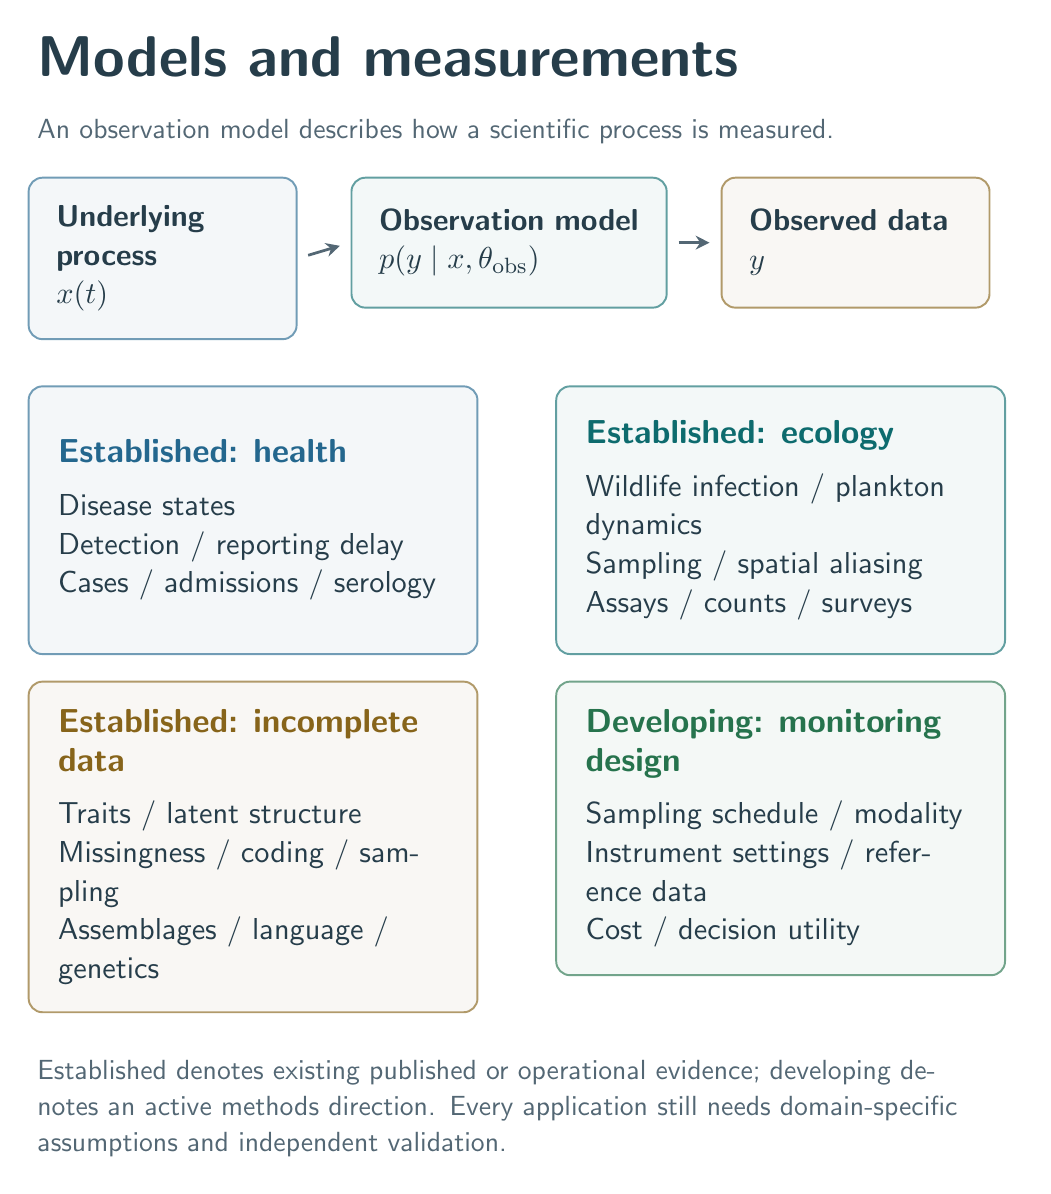
\begin{tikzpicture}
\heading{Models and measurements}{An observation model describes how a scientific process is measured.}
\node[panel=Blue,minimum width=3.4cm,text width=2.7cm,minimum height=1.65cm] (latent) at (0,0) {\textbf{Underlying process}\\\(x(t)\)};
\node[panel=Teal,minimum width=4cm,text width=3.3cm,minimum height=1.65cm] (obs) at (4.1,0) {\textbf{Observation model}\\\(p(y\mid x,\theta_{\mathrm{obs}})\)};
\node[panel=Gold,minimum width=3.4cm,text width=2.7cm,minimum height=1.65cm] (data) at (8.8,0) {\textbf{Observed data}\\\(y\)};
\draw[flow] (latent.east) -- (obs.west);
\draw[flow] (obs.east) -- (data.west);
\panel{a}{0}{-2.65}{Blue}{Established: health}{Disease states\\Detection / reporting delay\\Cases / admissions / serology}
\panel{b}{6.7}{-2.65}{Teal}{Established: ecology}{Wildlife infection / plankton dynamics\\Sampling / spatial aliasing\\Assays / counts / surveys}
\panel{c}{6.7}{-6.4}{Green}{Developing: monitoring design}{Sampling schedule / modality\\Instrument settings / reference data\\Cost / decision utility}
\panel{d}{0}{-6.4}{Gold}{Established: incomplete data}{Traits / latent structure\\Missingness / coding / sampling\\Assemblages / language / genetics}
\node[note] at (0,-11.1) {Established denotes existing published or operational evidence; developing denotes an active methods direction. Every application still needs domain-specific assumptions and independent validation.};
\end{tikzpicture}
\end{document}
